\documentclass[conference,letterpaper]{IEEEtran}
\IEEEoverridecommandlockouts
\usepackage[utf8]{inputenc}
\usepackage[T1]{fontenc}
\usepackage[spanish,es-nodecimaldot]{babel}
\usepackage{lmodern}
\usepackage{microtype}
\usepackage{amsmath,amssymb}
\usepackage{graphicx}
\usepackage{booktabs}
\usepackage{array}
\usepackage{url}
\usepackage[hidelinks]{hyperref}
\usepackage{balance}
\usepackage{cite}
\graphicspath{{figuras/}}
\interdisplaylinepenalty=2500
\renewcommand{\IEEEkeywordsname}{Palabras clave}
\newcommand{\rot}{\mathrm{R}}
\newcommand{\trans}{\mathrm{T}}
\newcommand{\norm}[1]{\left\lVert #1 \right\rVert}
\newcommand{\dd}{\mathrm{d}}
\newcommand{\atanDos}{\operatorname{atan2}}

% --- AUTORES: clase IEEEtran (tres integrantes) ---
% Editar nombres y correos aqui, manteniendo 3 bloques IEEE.
\title{Integración de Modelos Cinemáticos, Diferenciales\\
	y Dinámicos para Manipuladores (Hito 2)}
\author{
	\IEEEauthorblockN{Milagros Ortiz}
	\IEEEauthorblockA{Ingeniería Mecatrónica\\
		Universidad Católica Boliviana\\
		Tarija, Bolivia\\
		milagros.ortiz@ucb.edu.bo}
	\and
	\IEEEauthorblockN{Jesús Ibarra}
	\IEEEauthorblockA{Ingeniería Mecatrónica\\
		Universidad Católica Boliviana\\
		Tarija, Bolivia\\
		jesus.ibarra@ucb.edu.bo}
	\and
	\IEEEauthorblockN{Óscar Mancilla}
	\IEEEauthorblockA{Ingeniería Mecatrónica\\
		Universidad Católica Boliviana\\
		Tarija, Bolivia\\
		oscar.mancilla@ucb.edu.bo}
}

\begin{document}
	\maketitle
	\begin{abstract}
		Se presenta la implementación y validación computacional de un flujo integrado de robótica para el manipulador ABB IRB 120. Se emplea un modelo Denavit--Hartenberg de seis articulaciones, con una extensión de herramienta de \(95\,\mathrm{mm}\) como dato arbitrario de ejercicio. La cinemática inversa se resuelve mediante el desacoplamiento geométrico tipo Pieper, enumeración analítica de ramas y verificación de posición y orientación por cinemática directa. Una configuración admisible alimenta la planificación de trayectoria mediante segmentos lineales con mezclas parabólicas (LSPB), el Jacobiano geométrico del punto de herramienta (TCP) y un experimento independiente de singularidad de muñeca. Finalmente, los perfiles temporales de la segunda articulación excitan un modelo dinámico ilustrativo de un grado de libertad (1R), sin atribuir sus parámetros a los motores reales del ABB. Se documentan ocho casos de prueba: siete poses resueltas y una entrada inalcanzable correctamente rechazada. La reconstrucción del caso principal presenta errores de \(8.11\times 10^{-17}\,\mathrm{m}\) y \(1.30\times10^{-16}\,\mathrm{rad}\). El notebook resulta reproducible y distingue las comprobaciones numéricas de las limitaciones de validez física.
	\end{abstract}
	
	\begin{IEEEkeywords}
		Cinemática inversa, Pieper, ABB IRB 120, cinemática directa, LSPB, Jacobiano, singularidades, dinámica 1R, Jupyter.
	\end{IEEEkeywords}
	
	\section{Introducción}
	La ejecución de una tarea robótica requiere convertir una pose cartesiana deseada en una configuración articular realizable, describir su evolución temporal y examinar las velocidades y esfuerzos asociados. Estos problemas pertenecen a modelos distintos, pero deben estar conectados: una solución de cinemática inversa (IK) no es suficiente si no reproduce la pose mediante cinemática directa (FK), no cumple límites o no conduce a una trayectoria coherente.
	
	Se presenta un \emph{pipeline} integrado formado por IK analítica tipo Pieper, validación FK, trayectoria LSPB, Jacobiano y análisis de singularidades, y dinámica reducida 1R, con evidencia ejecutable en Python y reporte IEEE en \LaTeX{}~\cite{guia,proyecto}. El manipulador de referencia es el ABB IRB 120, de seis ejes; el modelo cinemático se conserva del Hito 1~\cite{abb,guiah1}.
	
	El aporte de este trabajo es la integración verificable de los cinco módulos, la explicitación de ramas singulares y límites, y la separación rigurosa entre resultados del manipulador y los del ejemplo dinámico pedagógico.
	
	\section{Metodología}
	
	\subsection{Modelo geométrico, cinemática inversa y validación}
	Se utiliza la convención Denavit--Hartenberg estándar,
	\begin{equation}
		{}^{i-1}T_i=R_z(\theta_i)T_z(d_i)T_x(a_i)R_x(\alpha_i),
		\label{eq:dh}
	\end{equation}
	con \(\theta_2=q_2-\pi/2\). Las longitudes empleadas se muestran en la Tabla~\ref{tab:dimensiones}. Los valores de geometría del manipulador son consistentes con el esquema dimensional oficial del IRB 120-3/0.6 de ABB~\cite{abb}, conservando los marcos adoptados en el Hito 1.
	
	\begin{table}[!b]
		\caption{Geometría del modelo y extensión de herramienta}
		\label{tab:dimensiones}
		\centering
		\footnotesize
		\begin{tabular}{@{}lll@{}}
			\toprule
			Parámetro & Valor & Procedencia / carácter \\
			\midrule
			\(d_1\) & \(0.290\,\mathrm{m}\) & Geometría ABB / Hito 1 \\
			\(a_2\) & \(0.270\,\mathrm{m}\) & Geometría ABB / Hito 1 \\
			\(a_3\) & \(0.070\,\mathrm{m}\) & Geometría ABB / Hito 1 \\
			\(d_4\) & \(0.302\,\mathrm{m}\) & Geometría ABB / Hito 1 \\
			\(d_6\) & \(0.072\,\mathrm{m}\) & Geometría ABB / Hito 1 \\
			\(\ell_{TCP}\) & \(0.095\,\mathrm{m}\) & Valor arbitrario \\
			\bottomrule
		\end{tabular}
	\end{table}
	
	\textbf{Convención de la herramienta.} Se añadió una herramienta rígida ideal cuya longitud puede elegirse arbitrariamente; en este ejercicio se fija \(\ell_{TCP}=0.095\,\mathrm{m}\) sobre el eje \(+z_6\). No es una dimensión de una herramienta comercial ABB ni un dato atribuido al fabricante. Las dimensiones de carcasa y dedos dibujadas en los apuntes son descriptivas; el notebook modela solo el desplazamiento del TCP, sin geometría de colisión de la pinza. La transformación correspondiente es
	\begin{equation}
		{}^6T_{TCP}=\begin{bmatrix}
			1&0&0&0\\0&1&0&0\\0&0&1&0.095\\0&0&0&1
		\end{bmatrix}.
		\label{eq:tcp}
	\end{equation}
	La cinemática del TCP se determina por
	\({}^0T_{TCP}(q)={}^0T_6(q){}^6T_{TCP}\).
	La pose de interés, \(T_d\), siempre corresponde al \emph{TCP} respecto de la base, y no directamente al marco 6. Antes de iniciar la IK se determina \(T_{06,d}=T_d({}^6T_{TCP})^{-1}\) y luego el centro de la muñeca:
	\begin{equation}
		p_W=p_{06,d}-d_6R_{06,d}\hat z,\qquad \hat z=[0,0,1]^\trans.
		\label{eq:pw}
	\end{equation}
	
	Para las primeras tres articulaciones se definen \(r=\sqrt{x_W^2+y_W^2}\), \(h=z_W-d_1\), \(L=\sqrt{a_3^2+d_4^2}\), \(\beta=\atanDos(d_4,a_3)\) y \(\delta=q_3+\beta\). La geometría conduce a
	\begin{align}
		C&=\frac{r^2+h^2-a_2^2-L^2}{2a_2L}=\cos\delta,\label{eq:C}\\
		\delta_{\pm}&=\atanDos\!\left(\pm\sqrt{1-C^2},C\right),\label{eq:delta}\\
		q_3&=\delta-\beta,\label{eq:q3}\\
		q_2&=\atanDos(\rho,h)-\atanDos(L\sin\delta,a_2+L\cos\delta),\label{eq:q2}
	\end{align}
	donde \(\rho=\pm r\) representa las dos ramas de base. Si \(|C|>1\) más allá de la tolerancia de redondeo, la pose se rechaza por inalcanzabilidad geométrica. Se calculan hasta cuatro ramas de posición no singulares. Cuando \(x_W=y_W=0\), el ángulo \(q_1\) pertenece a una familia continua; el algoritmo evalúa representantes obtenidos de fronteras trigonométricas, los límites y puntos interiores de sus intervalos, sin afirmar que esa selección sea globalmente óptima.
	
	La muñeca esférica se determina mediante \(R_{36}=R_{03}^\trans R_{06,d}\). Si \(\sin q_5\neq0\), las dos ramas de orientación se obtienen de
	\begin{align}
		s_5&=\pm\sqrt{r_{13}^2+r_{23}^2},\quad q_5=\atanDos(s_5,r_{33}),\\
		q_4&=\atanDos(-r_{23}/s_5,-r_{13}/s_5),\\
		q_6&=\atanDos(-r_{32}/s_5,r_{31}/s_5),
	\end{align}
	con reconstrucción matricial adicional de \(q_6\) para robustez cuando \(s_5\) es pequeño. La combinación de ramas de posición y orientación produce hasta ocho ramas geométricas regulares.
	
	Para \(q_5=0\), \(R_{36}=R_z(q_4+q_6)\) y la condición es \(q_4+q_6=\phi+2\pi k\), lo cual define una familia continua en lugar de un único par angular. La selección respeta los intervalos articulares y minimiza \((q_4-q_{4,i})^2+(q_6-q_{6,i})^2\) en cada intervalo factible. Para configuraciones regulares, la selección final minimiza
	\begin{equation}
		q_f=\arg\min_{q^{(k)}\in\mathcal A}\norm{q^{(k)}-q_i}_2,
		\label{eq:sel}
	\end{equation}
	donde \(\mathcal A\) contiene representantes que satisfacen los límites y verifican por FK la pose \emph{completa}. Se usan errores \(e_p=\norm{p(q)-p_d}_2\) y \(e_R\) angular obtenidos de la diferencia de rotaciones, aceptando \(e_p\le10^{-8}\,\mathrm{m}\) y \(e_R\le10^{-8}\,\mathrm{rad}\). El uso sistemático de \(\atanDos\) conserva los cuadrantes geométricos.
	
	Los límites de \(q\) empleados son los del IRB 120 tradicional~\cite{abb}; la Tabla~\ref{tab:limites} también incluye velocidades máximas oficiales, utilizadas \emph{solo como referencia comparativa}, sin convertirlas en certificación de una trayectoria en robot físico.
	
	\begin{table}[!b]
		\caption{Rangos y velocidades publicados por ABB~\cite{abb}}
		\label{tab:limites}
		\centering\footnotesize
		\begin{tabular}{@{}cccc@{}}
			\toprule
			Eje & Límite inferior & Límite superior & \(\dot q_{\max}\) \\
			& (grados) & (grados) & (grados/s) \\
			\midrule
			J1 & $-165$ & $165$ & 250 \\
			J2 & $-110$ & $110$ & 250 \\
			J3 & $-110$ & $70$ & 250 \\
			J4 & $-160$ & $160$ & 320 \\
			J5 & $-120$ & $120$ & 320 \\
			J6 & $-400$ & $400$ & 420 \\
			\bottomrule
		\end{tabular}
	\end{table}
	
	\subsection{Planificación de trayectoria LSPB}
	Para el tránsito entre \(q_i\) y \(q_f\) se adopta una duración común \(t_f=3.0\,\mathrm{s}\), reposo en ambos extremos y un factor \(k=1.125>1\) aplicado a la aceleración mínima triangular de cada articulación. Si \(\Delta q_j=q_{f,j}-q_{i,j}\), se obtiene
	\begin{equation}
		a_j=k\frac{4\Delta q_j}{t_f^2},\quad
		t_c=\frac{t_f}{2}\left(1-\sqrt{1-\frac{1}{k}}\right)=1\,\mathrm{s}.
		\label{eq:acel}
	\end{equation}
	El signo de \(a_j\) reproduce el sentido del desplazamiento, y \(\dot q_{c,j}=a_jt_c\). El perfil \(q_j(t)\) es
	\begin{equation}
		\begin{cases}
			q_{i,j}+\tfrac12a_jt^2,&0\le t<t_c,\\
			q_{i,j}+a_jt_c(t-\tfrac12t_c),&t_c\le t<t_f-t_c,\\
			q_{f,j}-\tfrac12a_j(t_f-t)^2,&t_f-t_c\le t\le t_f.
		\end{cases}
		\label{eq:lspb}
	\end{equation}
	Sus derivadas proporcionan \(\dot q(t)\) y \(\ddot q(t)\). Las articulaciones con \(\Delta q_j=0\) permanecen en reposo. El factor \(k\) hace real el discriminante, introduce un tramo de velocidad constante de \(1\,\mathrm{s}\) y sincroniza las seis articulaciones. La comprobación de factibilidad disponible abarca límites articulares de posición y comparación con velocidades nominales ABB, \emph{no} una cota de aceleración certificada por el fabricante; por tanto no se afirma ejecución segura en hardware sin validación adicional de actuadores, carga y control.
	
	\subsection{Jacobiano y singularidades}
	Para cada articulación revoluta, el Jacobiano geométrico del TCP se forma con el origen \(o_{j-1}\) y eje \(z_{j-1}\) expresados en la base:
	\begin{equation}
		J_j(q)=\begin{bmatrix}
			z_{j-1}\times(p_{TCP}-o_{j-1})\\z_{j-1}
		\end{bmatrix},\qquad
		\begin{bmatrix}v_{TCP}\\\omega_{TCP}\end{bmatrix}=J(q)\dot q.
		\label{eq:jac}
	\end{equation}
	Se verifica mediante diferencias centrales de FK, con perturbación angular de \(10^{-6}\,\mathrm{rad}\), en los bloques lineal y angular. Como comprobación analítica concreta, en la pose final principal \(p_{TCP}=[0.437,\,0,\,0.426827]^\trans\,\mathrm{m}\), \(o_0=0\) y \(z_0=[0,0,1]^\trans\). Por tanto,
	\begin{equation}
		J_1=\begin{bmatrix}z_0\times p_{TCP}\\z_0\end{bmatrix}
		=\begin{bmatrix}0&0.437&0&0&0&1\end{bmatrix}^{\!\trans},
		\label{eq:manualjac}
	\end{equation}
	que coincide con la primera columna numérica. El cálculo manual se amplió a las seis columnas en las hojas
	analíticas del equipo. Redondeando a tres decimales,
	la matriz completa en la configuración final es
	{\setlength{\arraycolsep}{2.8pt}
		\begin{equation}
			J(q_f)\simeq
			\begin{bmatrix}
				0 & .137 & -.097 & 0 & -.167 & 0\\
				.437 & 0 & 0 & .167 & 0 & 0\\
				0 & -.437 & -.302 & 0 & 0 & 0\\
				0 & 0 & 0 & 1 & 0 & 0\\
				0 & 1 & 1 & 0 & 1 & 0\\
				1 & 0 & 0 & 0 & 0 & -1
			\end{bmatrix}.
			\label{eq:jcompleto}
	\end{equation}}
	En la última entrada es esencial el signo negativo: el eje
	\(z_5\) apunta hacia \(-z_0\) en \(q_f\). La matriz coincide
	con la evaluación numérica de la función \texttt{jacobiano\_tcp}.
	
	Para no mezclar unidades de velocidad lineal y angular en el diagnóstico por valores singulares, se utiliza \(\bar J=[J_v/L_{\mathrm{ref}};J_\omega]\), con \(L_{\mathrm{ref}}=a_2=0.270\,\mathrm{m}\). El rango numérico cuenta los valores singulares \(\sigma_i>10^{-9}\sigma_{\max}\). La detección de singularidad se basa en \(\operatorname{rank}J<6\), no solamente en el determinante. Se examinan tanto la LSPB como una secuencia independiente \(q_5\to0\); esta última mantiene \(q_1=0^\circ\), \(q_2=30^\circ\), \(q_3=-30^\circ\) y \(q_4=q_6=0^\circ\). La velocidad cartesiana requerida es \([0,0,0,0,0,0.1]^\trans\), en unidades SI.
	
	\subsection{Modelo dinámico reducido 1R}
	Se usa el modelo de un eslabón rígido en plano vertical, con \(\theta\) referido a la vertical hacia abajo~\cite{dinamica}. Con energía cinética \(T=\tfrac12I_{\mathrm{eq}}\dot\theta^2\) y potencial \(V=mg\ell_c(1-\cos\theta)\), Euler--Lagrange conduce a
	\begin{equation}
		\tau(t)=I_{\mathrm{eq}}\ddot\theta(t)+mg\ell_c\sin\theta(t).
		\label{eq:torque}
	\end{equation}
	En este ensayo \(\theta(t)=q_2(t)\). Se adoptan \(I_{\mathrm{eq}}=0.25\,\mathrm{kg\,m^2}\), \(m=1.0\,\mathrm{kg}\), \(\ell_c=0.5\,\mathrm{m}\) y \(g=9.81\,\mathrm{m/s^2}\), como \textbf{parámetros numéricos ilustrativos del ejemplo de clase}, no como mediciones ni propiedades certificadas del robot ABB. La inercia es constante, no se modelan fricción ni acoplamientos, y el término de Coriolis es nulo bajo estas hipótesis. Se calculan y grafican separadamente \(\tau_{\mathrm{in}}=I_{\mathrm{eq}}\ddot\theta\), \(\tau_g=mg\ell_c\sin\theta\) y su suma.
	
	\subsection{Integración y reproducibilidad}
	La implementación utiliza un único notebook Jupyter con NumPy y Matplotlib. El flujo reutiliza resultados, sin resolver independientemente los módulos: \(T_d\to\) IK \(\to\) FK \(\to\) LSPB \(\to\) \(J(q(t))\) y singularidades \(\to\) \(\tau(t)\) del modelo 1R. Se mantienen unidades SI internamente (m, rad, s) y se presentan algunas gráficas en grados para su lectura. El registro de ocho casos se exporta a \texttt{resultados/registro\_pruebas.csv} y \texttt{resultados/registro\_pruebas.json}; el segundo conserva las poses objetivo y parámetros. La reproducción exacta requiere ejecutar todas las celdas en orden desde un kernel limpio y observar las advertencias de singularidad. No se requiere ROS, RViz ni Gazebo en este hito~\cite{guia}.
	
	\section{Resultados clave}
	\subsection{Ramas IK y validación FK}
	Para el caso principal se aplicó la pose objetivo
	\begin{equation}
		T_d=\begin{bmatrix}
			1&0&0&0.437\\
			0&-1&0&0\\
			0&0&-1&0.193+0.135\sqrt3\\
			0&0&0&1
		\end{bmatrix},
		\label{eq:pose}
	\end{equation}
	con longitudes en metros y \(q_i=[0,0,0,0,0,0]^\trans\). Se extrajeron ocho ramas geométricas regulares. La Tabla~\ref{tab:ramas} distingue las opciones geométricas y su admisibilidad: una rama geométrica, A++, cumple los límites (puede producir más de un representante equivalente por vueltas completas admisibles de J6). La regla de cercanía seleccionó \(q_f=[0,30,-30,0,90,0]^\trans\) grados.
	
	\begin{table*}[!t]
		\caption{Ocho ramas geométricas del caso principal (grados); reconstrucción FK y límites del modelo}
		\label{tab:ramas}
		\centering\footnotesize
		\begin{tabular}{@{}lrrrrrrrl@{}}
			\toprule
			Rama & $q_1$ & $q_2$ & $q_3$ & $q_4$ & $q_5$ & $q_6$ & $e_p$ (m) & Admisibilidad \\
			\midrule
			A++ & $0$ & $30.00$ & $-30.00$ & $0$ & $90.00$ & $0$ & $8.11\!\times\!10^{-17}$ & Cumple \\
			A+- & $0$ & $30.00$ & $-30.00$ & $-180$ & $-90.00$ & $-180$ & $8.11\!\times\!10^{-17}$ & Fuera: J4 \\
			A-+ & $0$ & $80.38$ & $-123.90$ & $0$ & $133.52$ & $0$ & $2.36\!\times\!10^{-16}$ & Fuera: J3, J5 \\
			A-- & $0$ & $80.38$ & $-123.90$ & $-180$ & $-133.52$ & $-180$ & $1.76\!\times\!10^{-16}$ & Fuera: J3, J4, J5 \\
			B++ & $-180$ & $-80.38$ & $-30.00$ & $-180$ & $159.62$ & $0$ & $1.12\!\times\!10^{-16}$ & Fuera: J1, J4, J5 \\
			B+- & $-180$ & $-80.38$ & $-30.00$ & $0$ & $-159.62$ & $-180$ & $8.52\!\times\!10^{-17}$ & Fuera: J1, J5 \\
			B-+ & $-180$ & $-30.00$ & $-123.90$ & $-180$ & $116.10$ & $0$ & $1.13\!\times\!10^{-16}$ & Fuera: J1, J3, J4 \\
			B-- & $-180$ & $-30.00$ & $-123.90$ & $0$ & $-116.10$ & $-180$ & $8.52\!\times\!10^{-17}$ & Fuera: J1, J3 \\
			\bottomrule
		\end{tabular}
	\end{table*}
	
	La FK del representante elegido reconstruyó el TCP con \(e_p=8.1097\times10^{-17}\,\mathrm{m}\) y \(e_R=1.2958\times10^{-16}\,\mathrm{rad}\), claramente por debajo de las tolerancias de aceptación. Los resultados de las ocho pruebas de regresión se resumen en la Tabla~\ref{tab:regresion}. Entre las siete poses aceptadas, el mayor error de posición fue \(2.4980\times10^{-16}\,\mathrm{m}\) (Regular A), y el mayor error angular, \(4.1500\times10^{-16}\,\mathrm{rad}\) (Regular B). El caso \emph{Fuera de alcance} se rechazó como corresponde. El indicador \texttt{OK} confirma cálculos y criterios de FK; \emph{no} significa ausencia de singularidad.
	
	\begin{table}[!t]
		\caption{Pruebas registradas y advertencias de singularidad}
		\label{tab:regresion}
		\centering\scriptsize
		\begin{tabular}{@{}p{0.31\columnwidth}lp{0.35\columnwidth}@{}}
			\toprule
			Caso & Estado & Rango ini./fin. y aviso \\
			\midrule
			Principal & OK & 5/6; singular al inicio \\
			Regular A & OK & 5/6; singular al inicio \\
			Regular B & OK & 5/6; singular al inicio \\
			Muñeca $q_5=0$ & OK & 5/5; extremos singulares \\
			Acoplamiento 60$^\circ$ & OK & 5/5; extremos singulares \\
			Fuera de alcance & Rech. & Sin trayectoria (correcto) \\
			Centro sobre eje & OK & 5/5; extremos singulares \\
			Eje y muñeca sing. & OK & 5/5; extremos singulares \\
			\bottomrule
		\end{tabular}
	\end{table}
	
	\subsection{Perfiles LSPB y límites de velocidad}
	El factor \(k=1.125\) y \(t_f=3\,\mathrm{s}\) originan transiciones en \(t=1\) y \(t=2\,\mathrm{s}\). La Tabla~\ref{tab:lspb} reúne las articulaciones que efectivamente se mueven en el ejemplo principal. Los valores calculados están por debajo de las velocidades máximas oficiales de J2, J3 y J5 de la Tabla~\ref{tab:limites}. Los perfiles satisfacen \(q(0)=q_i\), \(q(t_f)=q_f\), \(\dot q(0)=\dot q(t_f)=0\) y continuidad de \(q,\dot q\) en \(t_c,t_f-t_c\).
	
	\begin{table}[!t]
		\caption{Perfil principal: articulaciones móviles}
		\label{tab:lspb}
		\centering\footnotesize
		\begin{tabular}{@{}crrr@{}}
			\toprule
			Junta & $q_f$ ($^\circ$) & $a$ ($^\circ/s^2$) & $v_c$ ($^\circ/s$) \\
			\midrule
			J2 & $30$ & $15$ & $15$ \\
			J3 & $-30$ & $-15$ & $-15$ \\
			J5 & $90$ & $45$ & $45$ \\
			\bottomrule
		\end{tabular}
	\end{table}
	
	\begin{figure*}[!t]
		\centering
		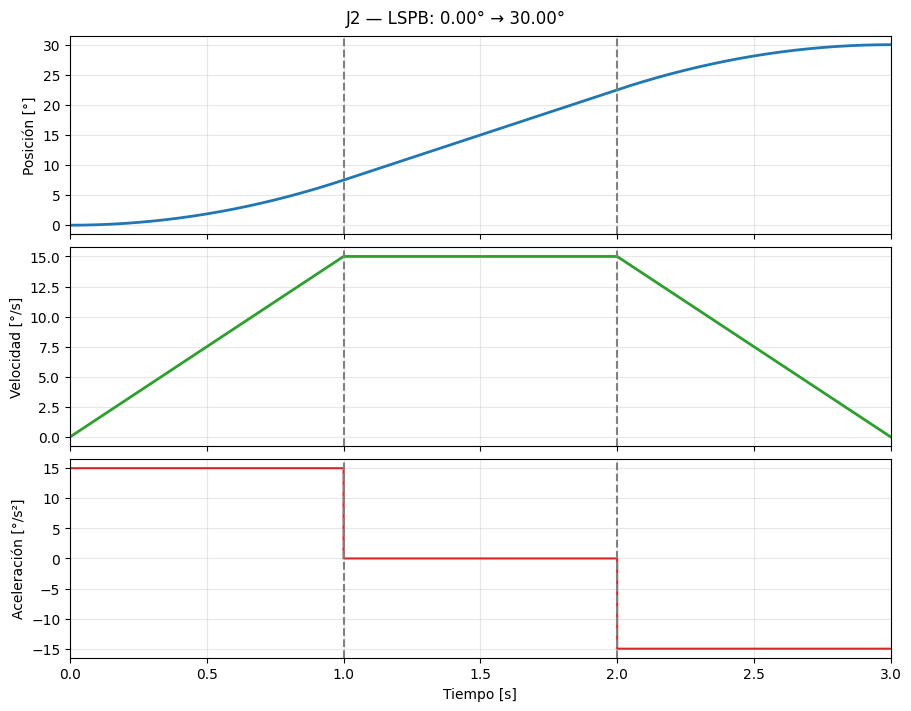
\includegraphics[width=0.48\textwidth]{lspb_j2.png}\hfill
		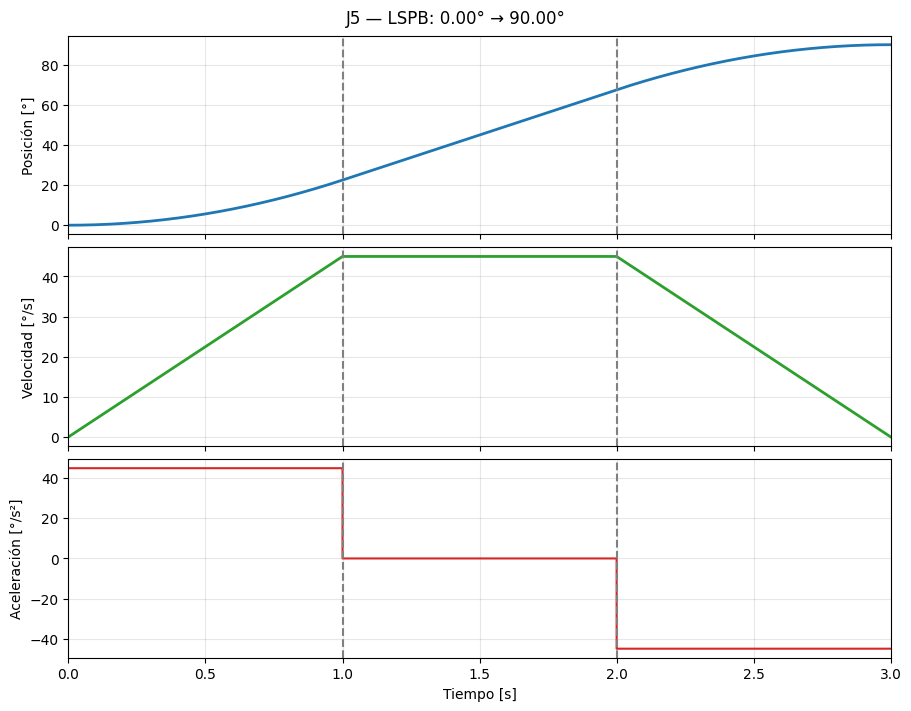
\includegraphics[width=0.48\textwidth]{lspb_j5.png}
		\caption{Posición, velocidad y aceleración LSPB de las articulaciones J2 (izquierda) y J5 (derecha), exportadas de las salidas originales del notebook. Las líneas discontinuas identifican los cambios de fase; la aceleración presenta saltos ideales.}
		\label{fig:lspb}
	\end{figure*}
	
	\paragraph{Comprobación cinemática simbólica.}
	Para la LSPB principal se verifica exactamente la relación
	\(q(t)=[0,\theta,-\theta,0,3\theta,0]^\trans\), con
	\(\theta(t)=q_2(t)\). Al usar la FK y
	\(\ell=d_6+\ell_{TCP}=0.167\,\mathrm{m}\), se llega a
	\begin{align}
		x_{TCP}(t)&=d_4+a_2\sin\theta+\ell\cos(3\theta),\\
		y_{TCP}(t)&=0,\nonumber\\
		z_{TCP}(t)&=d_1+a_2\cos\theta+a_3-\ell\sin(3\theta).
		\label{eq:tcp_simb}
	\end{align}
	De aquí se obtiene
	\(v_x=(a_2\cos\theta-3\ell\sin3\theta)\dot\theta\),
	\(v_z=(-a_2\sin\theta-3\ell\cos3\theta)\dot\theta\)
	y \(\omega_{TCP}=[0,3\dot\theta,0]^\trans\).
	Las expresiones concuerdan con las hojas analíticas y con \(J(q(t))\dot q(t)\), considerando
	\(\theta\) en radianes.
	
	\subsection{Verificación del Jacobiano y singularidad}
	La comparación del Jacobiano analítico con diferencias finitas en la configuración principal arrojó error máximo lineal de \(7.53\times10^{-11}\) y angular de \(1.33\times10^{-10}\), menores que el umbral de \(10^{-7}\). A lo largo de la LSPB principal se obtuvieron rangos 5 al inicio y 6 al final, con una muestra clasificada como singular entre las 601 evaluadas. Esto \emph{no} demuestra ausencia de singularidades entre muestras.
	
	\begin{figure}[!t]
		\centering
		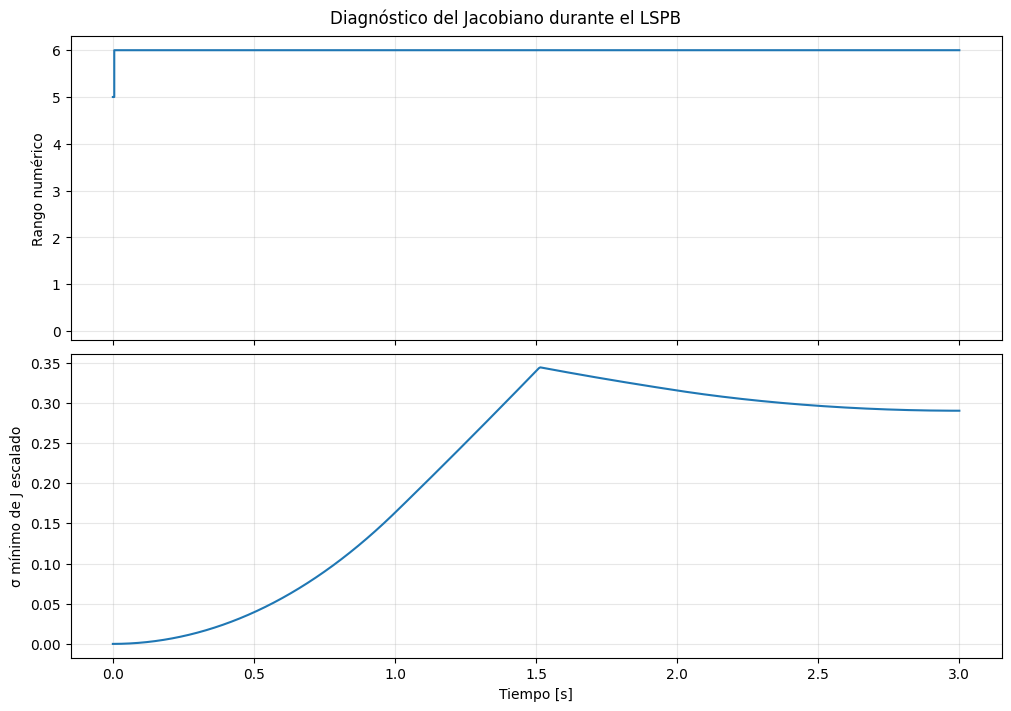
\includegraphics[width=\columnwidth]{rango_trayectoria.png}
		\caption{Rango numérico y mínimo valor singular del Jacobiano escalado a lo largo de la LSPB principal. La singularidad inicial se distingue del rango final 6.}
		\label{fig:rango}
	\end{figure}
	
	En el experimento independiente, al pasar \(q_5\) de \(30^\circ\) a \(0^\circ\), el menor valor singular de \(\bar J\) decrece y el rango cae a 5. Los ejes de J4 y J6 se alinean, con columnas coincidentes en la configuración final singular. Además, existe una condición de velocidad local \(v_y-0.604\,\omega_z=0\) para dicha configuración: la velocidad solicitada con \(\omega_z=0.1\,\mathrm{rad/s}\) produce una discrepancia de \(-0.0604\,\mathrm{m/s}\) respecto de esa restricción y, por ello, no puede imponerse exactamente.
	
	La demostración manual del defecto de rango admite
	el vector no nulo \(u=[0,0,0,1,0,-1]^\trans\) para el cual
	\(J(q_s)u=0\), con \(q_s=[0,30,-30,0,0,0]^\trans\) grados.
	Tras eliminar \(u_5=-u_2-u_3\), un menor de las ecuaciones
	restantes es
	{\setlength{\arraycolsep}{3pt}
		\begin{equation}
			\det\!\begin{bmatrix}.303827&.070000\\-.437&-.302\end{bmatrix}
			\simeq-0.061166\neq0.
			\label{eq:menor}
	\end{equation}}
	Por tanto, la nulidad es de dimensión uno y el rango es
	cinco, en coherencia con el experimento numérico.
	
	\begin{table}[!t]
		\caption{Aproximación a singularidad de muñeca}
		\label{tab:singularidad}
		\centering\footnotesize
		\begin{tabular}{@{}rrrr@{}}
			\toprule
			$q_5$ ($^\circ$) & Rango & $\sigma_{\min}(\bar J)$ & $\norm{\dot q}$ (rad/s)\\
			\midrule
			30 & 6 & $2.438\times10^{-1}$ & 0.3537\\
			5 & 6 & $4.076\times10^{-2}$ & 2.2364\\
			1 & 6 & $8.152\times10^{-3}$ & 11.1987\\
			0.1 & 6 & $8.152\times10^{-4}$ & 111.9935\\
			0.01 & 6 & $8.152\times10^{-5}$ & 1119.9358\\
			0 & 5 & $\simeq 0$ & No invertido\\
			\bottomrule
		\end{tabular}
	\end{table}
	
	\begin{figure}[!b]
		\centering
		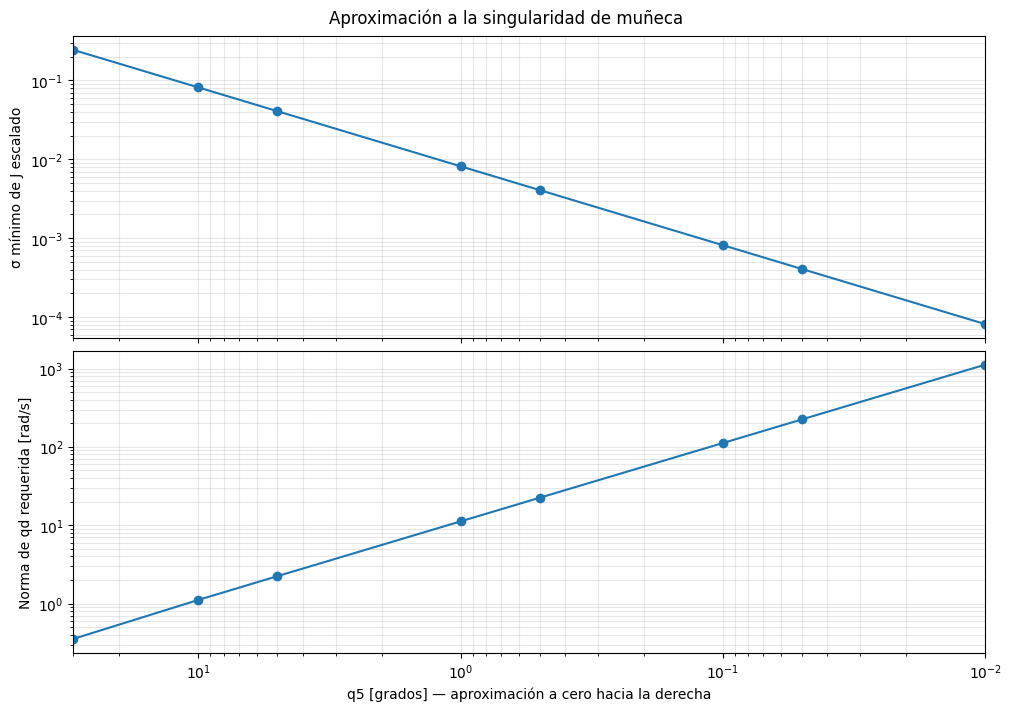
\includegraphics[width=\columnwidth]{singularidad_muneca.png}
		\caption{Valores singulares y norma de velocidad articular requerida conforme \(q_5\to0\). El punto de rango deficiente no se invierte numéricamente.}
		\label{fig:sing}
	\end{figure}
	
	\subsection{Torque del modelo reducido 1R}
	La trayectoria de J2 genera tres fases con \(\ddot\theta=+15,0,-15\,{}^\circ/\mathrm{s^2}\). Por tanto, la contribución inercial tiene amplitud \(|\tau_{\mathrm{in}}|=0.25(15\pi/180)=0.06545\,\mathrm{N\,m}\) en aceleración y frenado, y se anula durante el crucero. En cambio \(\tau_g=4.905\sin\theta\,\mathrm{N\,m}\) permanece distinta de cero cuando \(\theta\neq0\) incluso con velocidad constante.
	
	El \textbf{máximo absoluto entre las 601 muestras del movimiento} fue \(2.38705\,\mathrm{N\,m}\), registrado en \(t=3.0\,\mathrm{s}\), bajo la convención del notebook que todavía asigna la aceleración de frenado en el instante extremo. \textbf{Después de detenerse}, si se impone \(\ddot\theta=0\), el torque de sostén pasa a \(mg\ell_c\sin30^\circ=2.45250\,\mathrm{N\,m}\). No son magnitudes contradictorias: corresponden a estados de aceleración distintos en una frontera ideal con salto de \(\ddot\theta\). El par motor puede seguir siendo positivo durante el frenado: lo negativo es el par neto \(\tau-\tau_g=I_{\mathrm{eq}}\ddot\theta\), que origina la desaceleración.
	
	\begin{figure}[!b]
		\centering
		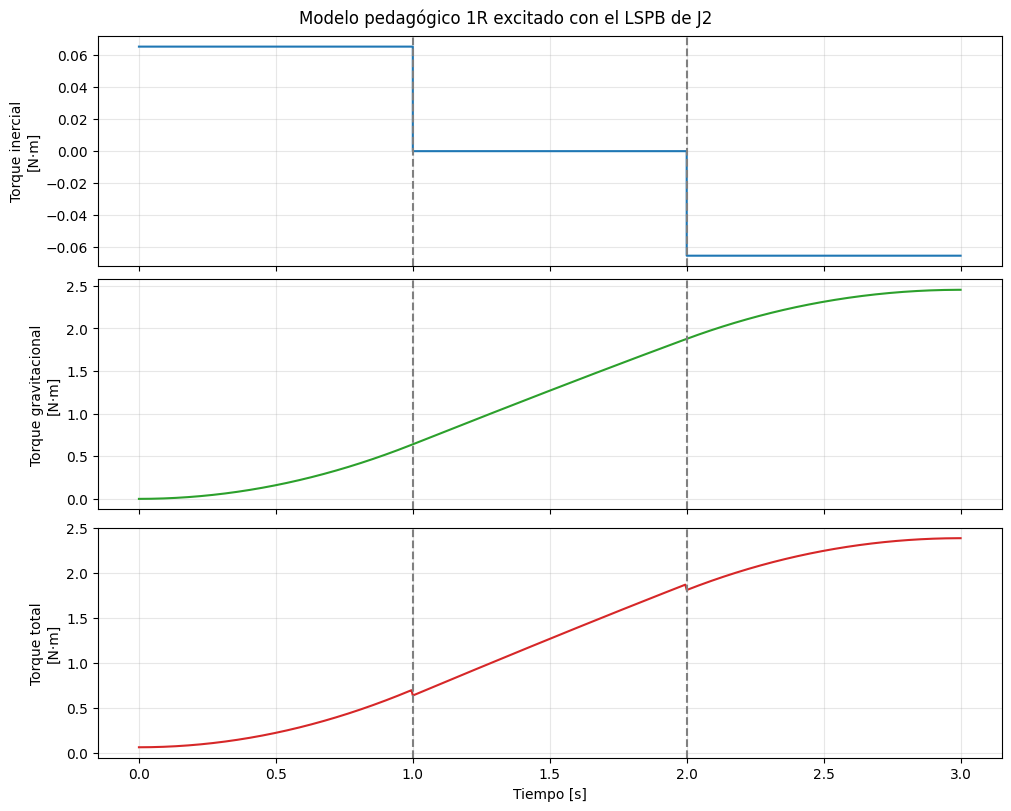
\includegraphics[width=\columnwidth]{torque_1r.png}
		\caption{Contribuciones inercial, gravitacional y total del ejemplo 1R, alimentadas por la trayectoria LSPB de J2. No representa torques reales de motores ABB.}
		\label{fig:torque}
	\end{figure}
	
	\section{Discusión}
	El cumplimiento de FK con errores próximos a la precisión de máquina respalda la coherencia \emph{interna} entre IK y FK, pero no constituye una medición de exactitud absoluta del robot físico. La presencia de ramas fuera de límites demuestra por qué el filtrado articular debe ser posterior a la obtención analítica de candidatos. Una pose impuesta en el momento puede resultar regular, singular, inadmisible por límites o fuera de alcance; cada condición exige una salida explicable, sin garantizar solución para poses imposibles.
	
	La LSPB evita discontinuidades de posición y velocidad y concentra esfuerzos inerciales en aceleración/frenado. El tramo de crucero conserva un torque gravitacional distinto de cero: \(\dot q=\mathrm{cte}\) no equivale a \(\tau=0\). Los saltos de aceleración en las fronteras son inherentes a la idealización LSPB y requerirían suavizado o comprobaciones adicionales antes de un uso real. Las velocidades verificadas son inferiores a las máximas publicadas, aunque faltan límites de aceleración y análisis de carga certificados para atribuir factibilidad física integral.
	
	La singularidad se define por pérdida de rango del Jacobiano y representa pérdida instantánea de direcciones de movimiento realizables. A medida que el menor valor singular disminuye, la resolución de una velocidad cartesiana fija puede exigir velocidades articulares enormes. No debe confundirse esta amplificación cinemática con \emph{torque infinito}: el torque depende del modelo dinámico, masas, inercias, gravedad y aceleraciones~\cite{dinamica,rubrica}. En particular, el ejemplo 1R es deliberadamente independiente del modelo dinámico completo del ABB. La herramienta de 95 mm fue autorizada para el ejercicio y no puede usarse como referencia industrial.
	
	En materia de reproducibilidad, la integración de resultados en CSV/JSON y la ejecución secuencial del notebook facilitan la auditoría. El registro de rango inicial/final requiere la advertencia adicional presentada en la Tabla~\ref{tab:regresion}; ninguna etiqueta \texttt{OK} certifica que todo el movimiento esté lejos de singularidades. La clasificación se realizó en muestras discretas y con tolerancia de rango explícita.
	
	\section{Conclusiones}
	Se implementó un flujo computacional coherente desde una pose TCP hasta una solución articular admisible, sus perfiles LSPB, las velocidades diferenciales y el torque de un ejemplo dinámico 1R. El caso principal seleccionó la rama A++ y verificó la pose completa con errores del orden de \(10^{-16}\). En ocho casos registrados se resolvieron siete objetivos y se rechazó correctamente una posición fuera del alcance geométrico.
	
	La planificación produjo perfiles sincronizados de \(3\,\mathrm{s}\), con \(t_c=1\,\mathrm{s}\) y reposo en ambos extremos. El Jacobiano fue contrastado con diferencias finitas y el experimento independiente reprodujo una pérdida de rango de 6 a 5 en \(q_5=0\), acompañada de amplificación de la velocidad articular solicitada. Finalmente, el cálculo 1R evidenció contribuciones inerciales y gravitacionales diferenciables, sin atribuir torques ilustrativos al ABB real.
	
	Se concluye que los resultados demuestran funcionamiento y reproducibilidad \emph{computacional} del pipeline para las pruebas efectuadas. Quedan delimitados los aspectos no certificados: aceleraciones y cargas reales, colisiones, garantía global de selección en familias axiales y evaluación de todas las posibles poses futuras de la defensa.
	
	\balance
	\begin{thebibliography}{00}
		\bibitem{siciliano} B. Siciliano, L. Sciavicco, L. Villani y G. Oriolo, \emph{Robotics: Modelling, Planning and Control}. Springer, 2009.
		\bibitem{guia} B. Quiroga Turdera, ``Guía Oficial y Rúbrica de Evaluación: Hito 2'', IMT-342, Universidad Católica Boliviana, Tarija, 2026, material docente.
		\bibitem{proyecto} B. Quiroga Turdera, ``Proyecto Computacional Integrado: Hito 2 -- Implementación y Validación de la Unidad II'', IMT-342, Universidad Católica Boliviana, 2026, material docente.
		\bibitem{rubrica} B. Quiroga Turdera, ``Rúbrica Oficial de Evaluación: Hito 2'', IMT-342, Universidad Católica Boliviana, 2026, material docente.
		\bibitem{dinamica} B. Quiroga Turdera, ``Dinámica Esencial de Manipuladores e Integración Hito 2'', Semana 9, Sesión 2, Universidad Católica Boliviana, 2026, material docente.
		\bibitem{abb} ABB Robotics, \emph{Product Specification -- IRB 120}, doc. 3HAC035960-001, rev. W, 2023, págs. 14 (dimensiones), 34 (rangos) y 36 (velocidades). Disponible en: \href{https://library.e.abb.com/public/429d251dbce44b049ba7d6107a422de0/3HAC035960\%20PS\%20IRB\%20120-en.pdf}{ABB Digital Library} (consulta: 22 oct. 2026).
		\bibitem{guiah1} B. Quiroga Turdera, ``Guía de Construcción URDF para el ABB IRB 120 (Hito 1)'', Universidad Católica Boliviana, 2026, material docente.
	\end{thebibliography}
\end{document}
